\section{Results and analysis}
To run the algorithm we used the same data used by the researchers. The fires occurred in Huzhong region located in
Mt. Daxing’anling at 10:40 local time on June 29, 2010. There was a total of 7 fire points in the region. The researchers reported
all the necessary parameters to calculate the objective functions. The only thing that was missing were the upper bounds to the number
of vehicles for each fire point ($U_i$), we used $10$ for all the points.\\
In table \ref{tab:our_solutions} we reported the results obtained after running 
the algorithm 4 consecutive times. The lowest calculated time to extinguish all
the fires is 6.17 hours, using all the vehicles, while the lowest number of
vehicles used is 29, that is the lower bound given by the authors, and the extinguish
time is 40.04 hours. In figure \ref{fig:pareto_results} these solutions are plot on a 2D graph with 
$f_1$ on the $x$ axis and $f_2$ on the $y$ axis. We can see that most of the solutions are concentrated 
between 5 and 20 hours for $f_1$ and these solutions cover almost all the values in $f_2$, so the results are satisfying. 
Our results are very similar to the ones found by the authors, however the pareto front in their experiment (Fig. \ref{fig:authors_results}) is very well distributed and 
all the runs produce very similar solutions, but we don't know if they used the same seed for the random number generator.
\newpage
\begin{table}
    \centering
    \caption{PRODUCED PARETO SOLUTIONS}
    \renewcommand{\arraystretch}{1.5}
    \begin{tabular}{ |c c c c c|  }
        \hline
        Runs & Solution Number & Scheduling schemes & $f_1$ (h) & $f_2$\\
        \hline
        \multirow{9}{*}{1} & 1 & $\{5, 4, 3, 8, 7, 6, 4\}$ & 8.25  & 37 \\
                           & 2 & $\{7, 3, 4, 8, 8, 6, 4\}$ & 6.17  & 40 \\
                           & 3 & $\{5, 3, 3, 7, 6, 5, 6\}$ & 11.83 & 35 \\
                           & 4 & $\{5, 3, 3, 7, 7, 6, 3\}$ & 12.76 & 34 \\
                           & 5 & $\{5, 2, 3, 8, 6, 4, 3\}$ & 33.38 & 31 \\
                           & 6 & $\{5, 3, 3, 7, 8, 6, 4\}$ & 9.06  & 36 \\
                           & 7 & $\{7, 3, 3, 8, 7, 6, 4\}$ & 7.31  & 38 \\
                           & 8 & $\{5, 2, 3, 6, 7, 5, 4\}$ & 19.33 & 32 \\
                           & 9 & $\{6, 2, 3, 7, 7, 5, 3\}$ & 15.87 & 33 \\
        \hline
        \multirow{12}{*}{2} & 1  & $\{6, 4, 3, 8, 7, 6, 4\}$ & 7.28  & 38 \\
                           & 2  & $\{6, 3, 3, 8, 8, 6, 5\}$ & 6.71  & 39 \\
                           & 3  & $\{6, 3, 3, 9, 7, 7, 5\}$ & 6.46  & 40 \\
                           & 4  & $\{5, 2, 3, 6, 6, 4, 3\}$ & 40.04 & 29 \\
                           & 5  & $\{5, 2, 3, 7, 6, 5, 3\}$ & 18.68 & 31 \\
                           & 6  & $\{5, 3, 4, 7, 6, 6, 4\}$ & 10.76 & 35 \\
                           & 7  & $\{5, 2, 3, 7, 6, 5, 4\}$ & 15.48 & 32 \\
                           & 8  & $\{5, 3, 3, 7, 8, 6, 5\}$ & 8.67  & 37 \\
                           & 9  & $\{5, 2, 3, 6, 6, 5, 3\}$ & 24.36 & 30 \\
                           & 10 & $\{5, 2, 3, 7, 7, 5, 5\}$ & 13.26 & 34 \\
                           & 11 & $\{5, 2, 3, 7, 7, 5, 4\}$ & 13.65 & 33 \\
                           & 12 & $\{5, 3, 3, 7, 7, 5, 6\}$ & 10.00 & 36 \\
        \hline
        \multirow{10}{*}{3} & 1  & $\{6, 4, 3, 8, 7, 6, 5\}$ & 6.89  & 39 \\
                           & 2  & $\{5, 3, 3, 7, 7, 5, 3\}$ & 13.74 & 33 \\
                           & 3  & $\{5, 2, 3, 6, 6, 5, 3\}$ & 24.36 & 30 \\
                           & 4  & $\{5, 3, 4, 7, 7, 6, 4\}$ & 8.93 & 36 \\
                           & 5  & $\{5, 2, 3, 8, 7, 5, 4\}$ & 12.66 & 34 \\
                           & 6  & $\{5, 3, 3, 9, 7, 7, 4\}$ & 7.82 & 38 \\
                           & 7  & $\{5, 2, 4, 6, 6, 5, 3\}$ & 23.73 & 31 \\
                           & 8  & $\{5, 2, 3, 8, 8, 5, 4\}$ & 12.16 & 35 \\
                           & 9  & $\{6, 3, 5, 8, 7, 6, 5\}$ & 6.38 & 40 \\
                           & 10 & $\{5, 4, 4, 7, 7, 6, 4\}$ & 8.60 & 37 \\
        \hline
        \multirow{10}{*}{4} & 1  & $\{5, 2, 3, 7, 6, 5, 3\}$ & 18.68  & 31 \\
                           & 2  & $\{5, 3, 3, 7, 6, 6, 3\}$ & 14.60 & 33 \\
                           & 3  & $\{5, 3, 3, 8, 7, 5, 4\}$ & 9.56 & 35 \\
                           & 4  & $\{6, 3, 4, 8, 8, 5, 4\}$ & 7.45 & 38 \\
                           & 5  & $\{5, 4, 3, 7, 7, 7, 4\}$ & 8.88 & 37 \\
                           & 6  & $\{6, 3, 3, 7, 8, 5, 4\}$ & 9.06 & 36 \\
                           & 7  & $\{6, 4, 3, 7, 8, 6, 5\}$ & 7.37 & 39 \\
                           & 8  & $\{6, 3, 3, 9, 8, 6, 5\}$ & 6.31 & 40 \\
                           & 9  & $\{5, 2, 3, 7, 7, 5, 5\}$ & 13.26 & 34 \\
                           & 10 & $\{5, 2, 3, 7, 6, 5, 4\}$ & 15.48 & 32 \\
        \hline
    \end{tabular}
    
    \label{tab:our_solutions}
\end{table}

\begin{figure}
    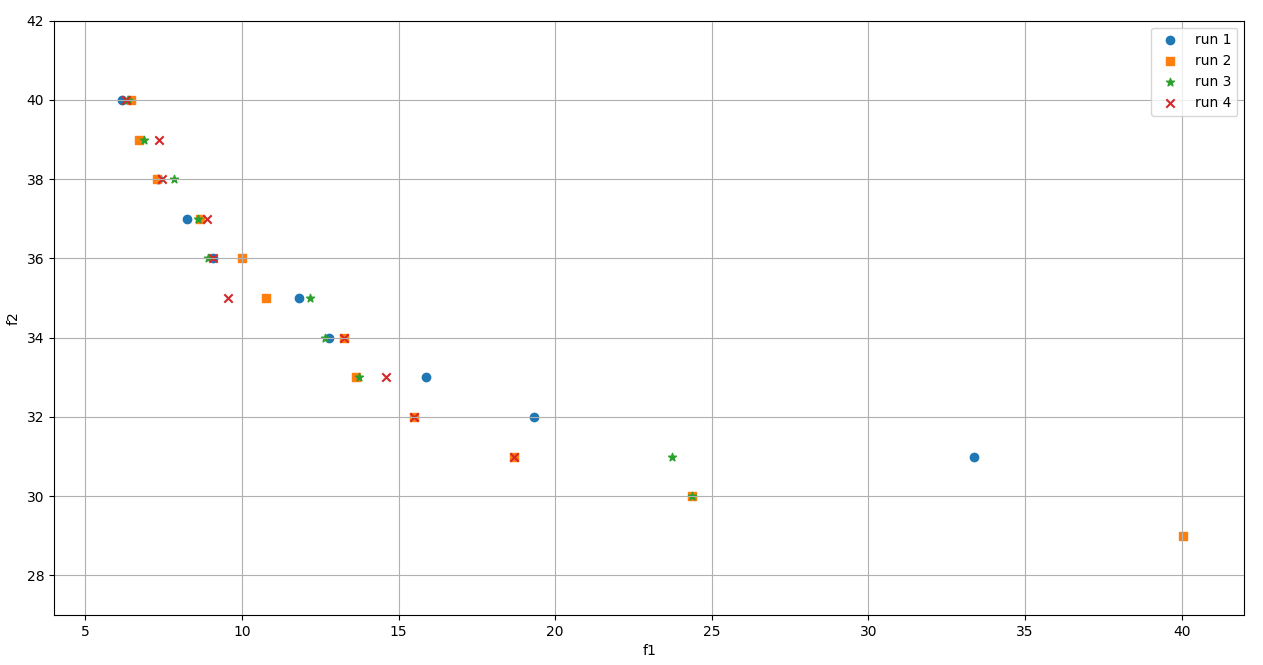
\includegraphics[width=\linewidth]{Images/our_results_4_runs.png}
    \caption{Our Pareto solutions}
    \label{fig:pareto_results}
\end{figure}

\begin{figure}
    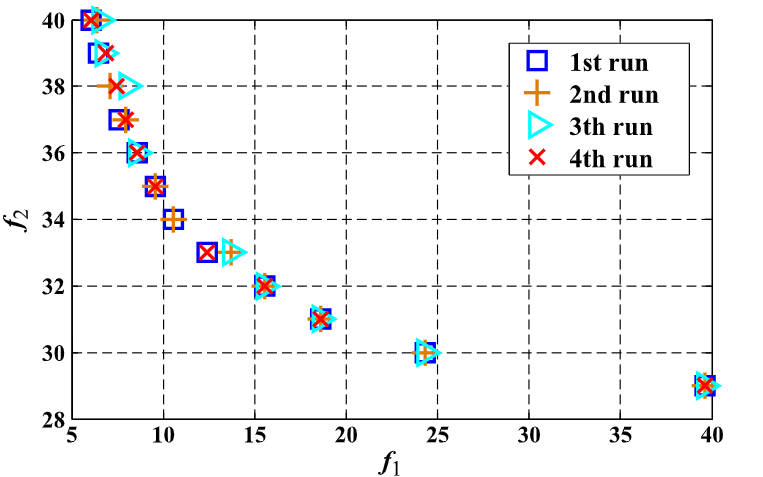
\includegraphics[width=\linewidth]{Images/authors_results.png}
    \caption{Authors' Pareto solutions}
    \label{fig:authors_results}
\end{figure}